\documentclass{standalone} % What kind of document this is
\usepackage{tikz} % Import the tikz package
\usetikzlibrary{automata, arrows.meta, positioning}
\tikzset{node distance=2.5cm, % Minimum distance between two nodes. Change if necessary.
  every state/.style={ % Sets the properties for each state
    semithick,
    fill=gray!10},
  initial text={}, % No label on start arrow
  double distance=2pt, % Adjust appearance of accept states
  every edge/.style={ % Sets the properties for each transition
    draw,
    ->,>=stealth, % Makes edges directed with bold arrowheads
    auto,
    semithick}}
\let\epsilon\varepsilon
\begin{document}
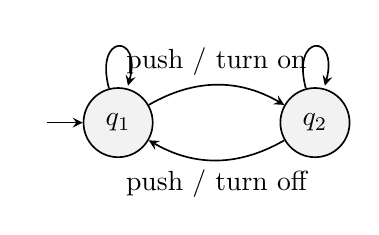
\begin{tikzpicture}
  \node[state without output, initial] (q1) {$q_1$};
  \node[state without output, right of=q1] (q2) {$q_2$};
  \draw (q1) edge[loop above] node {} (q1);
  \draw (q2) edge[loop above] node {} (q2);
  \draw (q2) edge[bend left] node {push / turn off} (q1);
  \draw (q1) edge[bend left] node {push / turn on} (q2);
\end{tikzpicture}
\end{document}
